% -*- TeX -*- -*- UK -*- -*- Soft -*-

\chapter{Regularization, Overfitting and Underfitting}
\label{sec:Regularization}

\section{The Bias-Variance Tradeoff}

This information is taken from \cite{DanielSaunders2017}.

Today's post is about the \textit{bias-variance} tradeoff, a well-known problem in machine learning which involves minimizing two sources of error which prevent supervised learning algorithms from generalizing well to new data. We'll discuss point estimation and statistical bias, variance (and their relationship with generalization), and consistency.

\subsection{Point Estimation}

From Deep Learning \cite{Goodfellow2016}: ``Point estimation is the attempt to provide the single `best' prediction of some quantity of interest.'' The quantity of interest may be a parameter, a vector of parameters, or even a function. The book uses the notation $\boldsymbol{\hat{\theta}}$ to denote a point estimate of a parameter $\boldsymbol{\theta}$.



Now, if $\{ \boldsymbol{x}^{(1)}, ..., \boldsymbol{x}^{(m)}\}$ is a set of \ac{IID} data samples, any function of the data
\begin{equation}
\boldsymbol{\hat\theta}_m = g(\boldsymbol{x}^{(1)}, ..., \boldsymbol{x}^{(m)})
\end{equation}
is considered a \textit{point estimate} or a \textit{statistic} of the data. This definition doesn't require that $g$ returns a good estimate of $\boldsymbol{\theta}$, or even that the range of $g$ is the same as the allowable values of $\boldsymbol{\theta}$; in this sense, it allows the designer of the estimator a great deal of flexibility. We consider a good estimator to be a function $g$ whose output is close to the true $\boldsymbol{\theta}$ which generated the dataset $\{ \boldsymbol{x}^{(1)}, ..., \boldsymbol{x}^{(m)} \}$.

In this discussion, we take the frequentist view on statistics: the true parameter value $\boldsymbol{\theta}$ is fixed but unknown, and the statistic $\boldsymbol{\hat\theta}$ is a function of the dataset. Since the data is generated from a random process parametrized by $\boldsymbol{\theta}$, any function of the dataset is random; therefore, the estimator $\boldsymbol{\hat\theta}$ is a random variable.

Point estimation can also refer to estimation of the relationship between input (explanatory) and output (dependent) variables; this is commonly referred to as function estimation. We now try to predict a variable $\boldsymbol{y}$ given an input vector $\boldsymbol{x}$. We assume there is a function $f(\boldsymbol{x})$ which captures the approximates the relationship between the two; e.g., we might assume that $\boldsymbol{y} = f(\boldsymbol{x}) + \boldsymbol{\epsilon}$, where $\boldsymbol{\epsilon}$ is the part of $\boldsymbol{y}$ which cannot be predicted from $\boldsymbol{x}$. In function estimation, we wish to approximate $f$ with a model or estimator $\hat f$. In this sense, function estimation is the same as point estimation, in which the estimated $\hat f$ is simply a point estimate in function space.

We can now review the most commonly studied properties of point estimators and discuss what they imply about these estimators.

\subsection{Bias}


Here, we are referring to statistical bias; that is, ``the difference between this estimator's expected value and the true value of the parameter being estimated'' \cite{wikipediaBiasofanestimator2019}. More formally, this is defined as:
\begin{equation}
\text{bias}(\boldsymbol{\hat\theta}_m) = \mathbb{E}[\boldsymbol{\hat\theta}_m] - \boldsymbol{\theta},
\end{equation}

where the expectation $\mathbb{E}[]$ is taken over the dataset (viewed as samples of a random variable) and $\boldsymbol{\theta}$ is the true value of the estimated parameter $\boldsymbol{\theta}$, used to define the data generating distribution. We call an estimator unbiased if $\text{bias}(\boldsymbol{\hat\theta}_m) = 0$, implying that its expected value, $\mathbb{E}[\boldsymbol{\hat\theta}_m] = \boldsymbol{\theta}$. An estimator is called asymptotically biased if $\text{lim}_{m \rightarrow \infty} \text{bias}(\boldsymbol{\hat\theta})_m = 0$, implying $\text{lim}_{m \rightarrow \infty} \mathbb{E}[\boldsymbol{\hat\theta}_m] = \boldsymbol{\theta}$.




\subsection{Variance and Standard Error}

We may also wish to consider how much we expect our estimator to vary as a function of the data sample. Just as we may compute the expectation of an estimator to determine its bias, we may also compute its variance, given by:

\begin{equation}
\text{Var}(\boldsymbol{\hat\theta}),
\end{equation}
where the random variable is the dataset. The square root of the variance is called the standard error, denoted by $\text{SE}(\boldsymbol{\hat\theta})$.

The variance or standard error of an estimator is a measure of much we expect the output of our estimator to vary as a function of independent resampling of data from the data generating distribution. Just as we might like an estimator to exhibit low bias, we might also want it to have low variance.

When we compute any statistic using a finite number of data samples, our estimate of the true parameter will always be uncertain, in the sense that we could have obtained different samples from the data generating distribution whose statistics would be different. Therefore, the expected degree of variation in an estimator is a source of error we would like to quantify.

The standard error of the mean is given by

\begin{equation}
\text{SE}(\hat\mu) = \sqrt{\text{Var}\left[\frac{1}{m}\sum_{i=1}^{m} x^{(i)}\right]} = \frac{\sigma}{\sqrt{m}},
\end{equation}
where $\sigma^2$ is the true variance of the samples $x^{(i)}$. The standard error is often estimated by using an estimate of $\sigma$; however, neither the square root of the sample variance nor the square root of the unbiased estimator of the variance is an unbiased estimated of the standard error. Both tend to underestimate the true standard deviation, yet are still commonly used in practice. For large $m$, the square root of the unbiased estimate provides a reasonable approximation.

The standard error of the mean can be useful for machine learning experiments. We often estimate the generalization error by computing the sample mean of the error on the test dataset, where the number of data samples in the set determines this estimate's accuracy. Using the central limit theorem, which tells us that the mean will be approximately distributed as a normal distribution, we can use the standard deviation to compute the probability that the true expectation falls in any given interval. For example, the 95\% confidence interval centered on the mean $\hat\mu_m$ is

\begin{equation}
(\hat\mu_m - 1.96 \text{SE}(\hat\mu_m),\hat\mu_m + 1.96 \text{SE}(\hat\mu_m))
\end{equation}
under the normal distribution with mean $\hat\mu_m$ and variance $\text{SE}(\hat\mu_m)^2$. In machine learning experiments, it is typical to say that algorithm A is better than algorithm B if the upper bound of the 95\% confidence interval for the error of algorithm A is less than the lower bound of the 95\% confidence interval for the error of algorithm B.


\subsection{Trading off Bias and Variance to Minimize Mean Squared Error}

Bias and variance measure two different sources of an estimator's error: bias measures the expected deviation from the true value of the function or parameter, and variance measures the deviation from the expected estimator value that any given sampling of from the data generating distribution is likely to cause.

How do we choose between two estimators, one with more bias and one with more variance? The most common way to settle this trade-off is by using cross-validation \cite{wikipediaCrossvalidation2019}, in which the training data is partitioned into $k$ equally subsets, each of which is ``held out'' to use as validation data in a series of training, validation ``rounds''. The results from evaluating the estimator on the validation data in each round is averaged to produce a estimated generalization error.

Alternatively, we may use the \ac{MSE} to compare estimators:

\begin{equation}
\text{MSE} = \mathbb{E}[(\boldsymbol{\hat\theta}_m - \boldsymbol{\theta})^2]
= \text{Bias}(\boldsymbol{\hat\theta}_m)^2 + \text{Var}(\boldsymbol{\hat\mu}).
\end{equation}
The \ac{MSE} measures the overall expected deviation, in the sense of squared errors, between the estimator and the true value of the parameter $\boldsymbol{\theta}$. From the above equation, the \ac{MSE} incorporates both the bias and variance in a natural way. Desirable estimators are those with small \ac{MSE}, and small bias and variance components in turn.

The relationship between bias and variance is closely related to the machine learning concepts of overfitting, underfitting, and capacity. When generalization error is measure by \ac{MSE}, where bias and variance are meaningful components, increasing model capacity tends to lead to an increase in variance and decrease in bias. This is illustrated in the figure, where we see a U-shaped generalization error curve as a function of model capacity.
\begin{marginfigure}
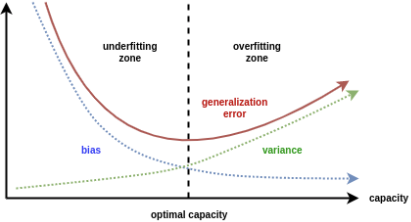
\includegraphics{ch13-snip01}
\end{marginfigure}



\subsection{Consistency}

So far, we've discussed useful properties of estimators given a training dataset of fixed size. We are usually interested in the behavior of the estimator as the size of this dataset grows. We typically want our point estimates to converge to the true value(s) of the corresponding parameter(s) as the number of data samples $m$ in our dataset grows. More formally, we want

\begin{equation}
\text{plim}_{m \rightarrow \infty} \boldsymbol{\hat\theta}_m = \boldsymbol{\theta},
\end{equation}
where $\text{plim}$ denotes convergence in probability; i.e., for any $\epsilon > 0, P(|\boldsymbol{\hat\theta}_m - \boldsymbol{\theta}| > \epsilon) \rightarrow 0$ as $m \rightarrow \infty$. This condition is known as consistency (sometimes known as weak consistency).

Consistency guarantees that the bias induced by the estimator diminishes as the number of training samples grows. The reverse is not true: asymptotic unbiasedness does not imply consistency, meaning there exist unbiased estimators which are not consistent.


\clearpage
\section{Regularization and Geometry}

The information in this section was originally taken from \cite{MinhPham2019,AnujaNagpal2017}.

\subsection{Bias-Variance Tradeoff}

When we perform statistical modeling, the goal is not to select a model that fits all the training data points and obtain the smallest error on the training data. The objective is to give the model the ability to generalize well on new and unseen data.
The grapphic shows the interplay between bias and variance, contributing to generalization error \cite{DanielSaunders2017}
\begin{marginfigure}
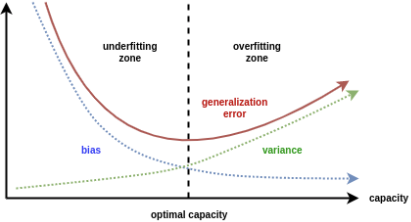
\includegraphics{ch13-snip01}
\end{marginfigure}

As more and more parameters are added to a model, the complexity of the model increases, i.e., it can fit more noise in training data and leads to overfitting. This means that we are increasing the variance and decreasing the bias of the model. From the figure above, if we keep raising the model's complexity, the generalization error will eventually pass the optimal spot and continue to increase.

To conclude, if our model complexity exceeds the optimal point, we risk falling into the overfitting zone; while if the complexity falls short of the optimal point, we are in the underfitting zone.

Regularization is a technique that helps prevent the statistical model from falling into the overfitting zone. It does so by hindering the complexity of the model.

\subsection{Regularization}

\newthought{Linear Regression}

This is the equation for a simple linear regression.
\begin{equation}
\hat{Y}=\beta_{0}+\beta_{1} X
\end{equation}
Our goal is to find the set of beta to minimize the \ac{RSSqr}.
\begin{equation}
\textrm{RSS}=\sum_{i=1}^{n}\left(y_{i}-\left(\beta_{0}+\beta_{1} x_{i}\right)\right)^{2}
\end{equation}



\newthought{L2 Regularization}

A regression model that utilizes L2 regularization is also called Ridge Regression. In terms of Linear Regression, instead of just minimizing the \ac{RSSqr}, we add another piece to the game by having a constraint for the betas.

\begin{equation}
\beta_{0}^{2}+\beta_{1}^{2} \leq s
\end{equation}
$s$ can be understood as a budget for the betas. If you want to make one of the first beta big, the second beta has to be small and vice versa. This becomes a competition and as we have more betas, the unimportant ones will be forced to be small.
\begin{marginfigure}
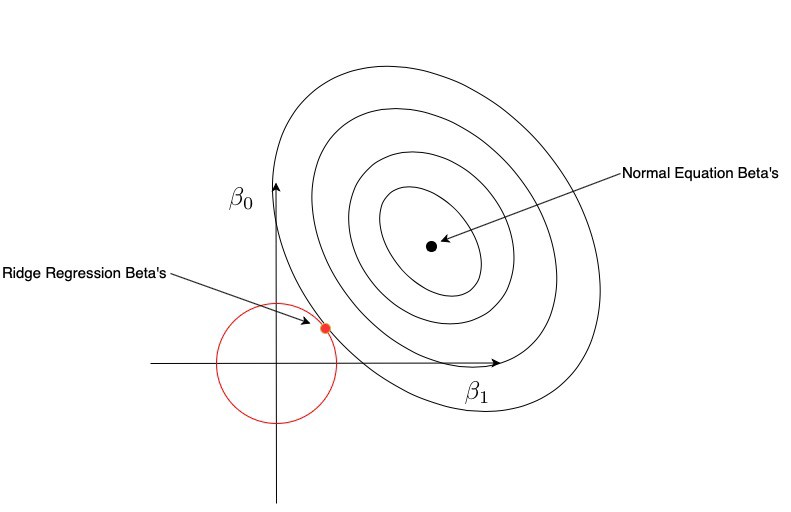
\includegraphics{ch13-snip02}
\end{marginfigure}
Due to the square term, the \ac{RSSqr} equation actually gives us the geometry of an ellipse. The black point is the set of betas using the normal equation, i.e., without regularization. The red circle contains all the sets of betas that we can ``afford.'' The red point is the final betas for Ridge Regression, which is closest to the black point while in our budget. The red point will always be on the boundary of the constraint. The only time that you attain a red point inside the constraint is when the solution for the normal equation, i.e., the solution for Linear Regression without regularization, already satisfies the constraint.

Ridge regression adds squared magnitude of coefficient as penalty term to the loss function.
\begin{equation}
\sum_{i=1}^{n}\left(y_{i}-\sum_{j=1}^{p} x_{i j} \beta_{j}\right)^{2}+\lambda \sum_{j=1}^{p} \beta_{j}^{2}
\end{equation}
Here, if $\lambda$ is zero then you can imagine we get back ordinary least squares. However, if $\lambda$  is very large then it will add too much weight and it will lead to under-fitting. Having said that it's important how $\lambda$  is chosen. This technique works very well to avoid over-fitting issue.


\newthought{L1 Regularization}

A regression model that utilizes L1 regularization is also called Lasso (Least Absolute Shrinkage and Selection Operator) Regression. The goal of Lasso is similar to Ridge with the exception that the constraint becomes:
\begin{equation}
\left|\beta_{0}\right|+\left|\beta_{1}\right| \leq s
\end{equation}
Lasso also provides us with a beautiful geometry that comes with unique properties.
\begin{marginfigure}
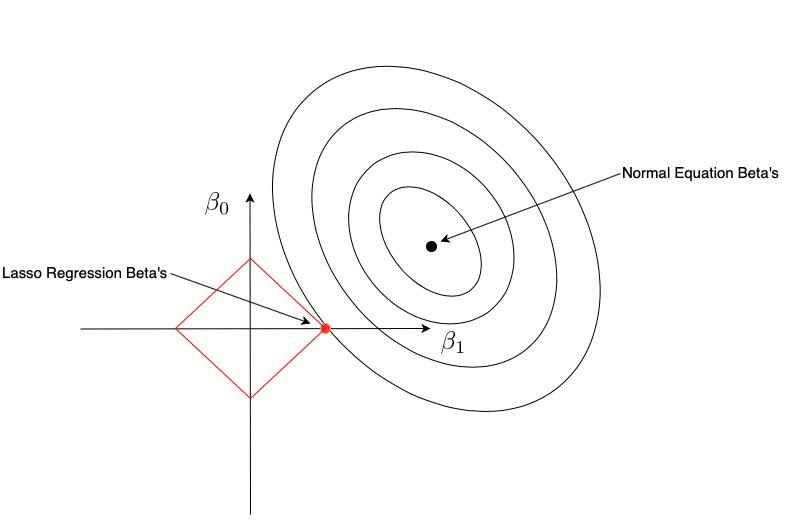
\includegraphics{ch13-snip03}
\end{marginfigure}

The set of betas that we can  ``afford'' with L2 regularization lies within a diamond. The red point is at the corner of the diamond, which sets one of the betas to 0.
What if the red point is on the edge of the diamond instead, i.e., the ellipse touches the diamond on the edge? Hence, neither of the betas will be 0. However, the diamond in 2-D space is a special case where neither of the betas becomes 0 if the red point is on the edge.

Lasso Regression (Least Absolute Shrinkage and Selection Operator) adds absolute value of magnitude of coefficient as penalty term to the loss function.
\begin{equation}
\sum_{i=1}^{n}\left(Y_{i}-\sum_{j=1}^{p} X_{i j} \beta_{j}\right)^{2}+\lambda \sum_{j=1}^{p}\left|\beta_{j}\right|
\end{equation}
Again, if $\lambda$ is zero then we will get back ordinary least squares whereas a very large value will make coefficients zero hence it will under-fit.

The key difference between these techniques is that Lasso shrinks the less important feature's coefficient to zero thus, removing some feature altogether. So, this works well for feature selection in case we have a huge number of features.

\newthought{L1 Regularization with 3 parameters}

Let us consider the Lasso case where we have 3 betas. The geometry for the constraint becomes a 3-D shape.
\begin{marginfigure}
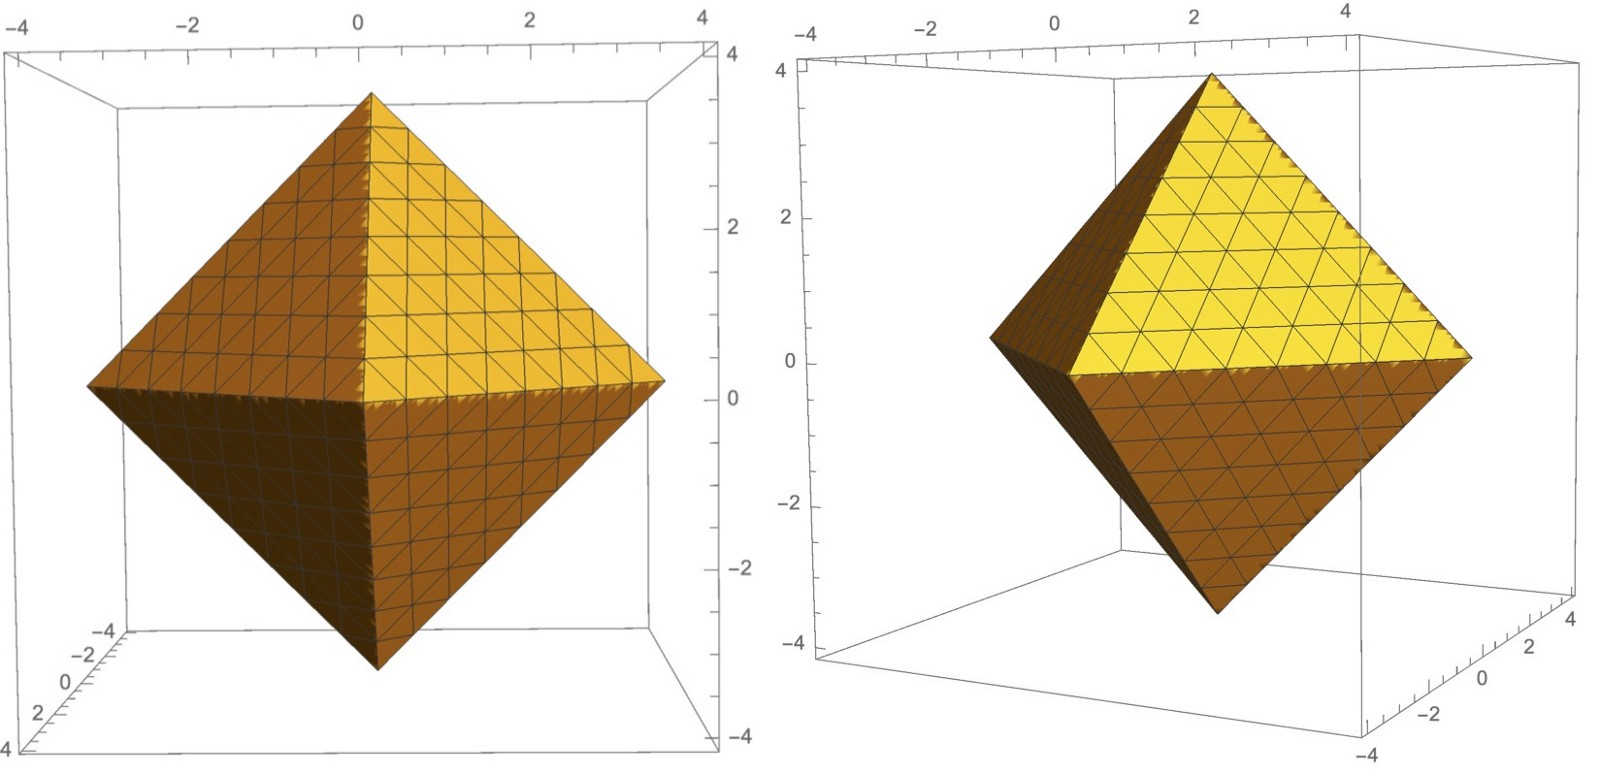
\includegraphics{ch13-snip04}
\end{marginfigure}

The figure above consists of 6 vertices and 8 edges. If the red point lies on an edge, one beta will be set to 0. If it lies on a vertices, two betas will be set to 0. As the dimension increases, the number of vertices and edges increases as well, making it more likely that the ellipse will be in contact with the diamond on one of those places. That being said, Lasso tends to work better in higher dimension.

\newthought{Differences between L1 and L2 Regularization}

Ridge regression is an extension for linear regression that enforces the betas coefficients to be small, reducing the impact of irrelevant features. This way the statistical model will not fit all the noise in the training data and fall into the overfitting zone.

Lasso regression bring some unique properties to the table because of its beautiful geometry. Some of the betas will be set to 0, giving us a sparse output. We can also use Lasso for feature selection. While feature selection techniques such as Best Subset, Forward Stepwise or Backward Stepwise may be time inefficient, Lasso will converge faster to the final solution.

\subsection{Conclusion}

A statistical model that with high complexity may be prone to overfitting. In this article, I introduced two regularization techniques to discourage the model from fitting all the noise in the training data. Moreover, I explained their properties and differences with the help of geometry.

Traditional methods like cross-validation, stepwise regression to handle overfitting and perform feature selection work well with a small set of features but these L1 and L2 regularization techniques are a great alternative when we are dealing with a large set of features.


